\documentclass{UoNMCHA}
\usepackage[authoryear]{natbib}
\usepackage{array,booktabs} % For nice tables
\usepackage{amsmath,amsfonts,amssymb} % For nice maths
\usepackage{color}
\usepackage{multicol}
\usepackage{enumerate}
\usepackage{listings}

\usepackage{subfig}
\usepackage{hyperref}
\usepackage[parfill]{parskip}   % For replacing paragraph indenting with a newline instead
\usepackage{float}
\newif\ifcomment
\commenttrue
\commentfalse
\raggedbottom
% Number equations per section
\numberwithin{equation}{section}

\hypersetup{
%    bookmarks=true,         % show bookmarks bar?
%    unicode=false,          % non-Latin characters in AcrobatÕs bookmarks
%    pdftoolbar=true,        % show AcrobatÕs toolbar?
%    pdfmenubar=true,        % show AcrobatÕs menu?
%    pdffitwindow=false,     % window fit to page when opened
%    pdfstartview={FitH},    % fits the width of the page to the window
%    pdftitle={My title},    % title
%    pdfauthor={Author},     % author
%    pdfsubject={Subject},   % subject of the document
%    pdfcreator={Creator},   % creator of the document
%    pdfproducer={Producer}, % producer of the document
%    pdfkeywords={keyword1} {key2} {key3}, % list of keywords
%    pdfnewwindow=true,      % links in new window
    colorlinks=true,       % false: boxed links; true: colored links
    linkcolor=blue,          % color of internal links
    citecolor=blue,        % color of links to bibliography
%    filecolor=magenta,      % color of file links
    urlcolor=blue           % color of external links
}

\definecolor{light-gray}{gray}{0.95}
\definecolor{myblue}{RGB}{20,105,176}
\definecolor{myorange}{RGB}{255,140,0}
\definecolor{mygrey}{RGB}{64,64,64}
\definecolor{MATLABKeyword}{rgb}{0,0,1}
\definecolor{MATLABComment}{rgb}{0.1328125,0.54296875,0.1328125}
\definecolor{MATLABString}{rgb}{0.625,0.125,0.9375}

\lstset{language=Matlab,
    basicstyle=\small\ttfamily,
    keywordstyle=\color{MATLABKeyword},
    %identifierstyle=,
    commentstyle=\color{MATLABComment},
    stringstyle=\color{MATLABString},
    numberstyle=\tiny,
    %numbers=left,
    basewidth=0.5em}
\lstset{
language=C,
numbers=none,
xleftmargin=1cm,
frame=tblr,
classoffset=0,
morekeywords={r0,r1,r2,r3,r4,r5,r6,r7,r8,r9,r10,r11,r12,r13,r14,r15},keywordstyle=\color{myblue},
classoffset=1,
morekeywords={ldr,srt,sub,cmp,it,bgt,b,str},	keywordstyle=\color{myorange},
classoffset=0,
commentstyle=\color{MATLABComment},
breaklines=true,
postbreak=\space //...
}





\firstpage{1}    % Set page number for first page
\UoNMCHAreportNo{ELEC1710 } %Report number
\UoNMCHAyear{ }   % Year
\shorttitle{ELEC1710 - Lab 4} %For odd pages
%%%%%%%%%%%%%%%%%%%%%%%%%%%%%%%%%%%%%%%%%%%%%%%%%%%%
\begin{document}
\title{Lab 4:\\Introduction to Microcontroller Programming \\ \ \\
{\small ELEC1710    \\ 
}}
%\author[UoNMCHA]{Student Name}
%\address[UoNMCHA]{
%Student of Mechatronics Engineering,\\
%The University of Newcastle, Callaghan, NSW 2308, AUSTRALIA \\
%Student Number: 3...... \\
%E-mail: \href{mailto:First.Last@uon.edu.au}{\textsf{First.Last@uon.edu.au}}}
%%%%%%%%%%%%%%%%%%%%%%%%%%%%%%%%%%%
\maketitle
\onecolumn

\vspace{-5mm}

\section{Introduction}

In this lab you will learn how to compile and debug code on the STM32F103C8T6 development board within the System Workbench development environment.

System Workbench is a free and open source software package which combines the Eclipse IDE (integrated development environment) with the GNU compiler toolchain (compiler, linker, assembler, etc) and comes pre-configured for STM32 software development.

It is available for download at \url{http://openstm32.org}, a free registration is required prior to download. The website also hosts a wiki and forums which can be useful sources of information, especially when encountering errors.

In this lab your primary tasks are as follows:

\begin{enumerate}
    \item Load a project into System Workbench
    \item Configure the debugging environment
    \item Compile the project
    \item Debug the code using various execution control tools
\end{enumerate}

\section{Knowledge Reference}

\begin{enumerate}
    \item Use of System Workbench is covered in a video on Blackboard. \textbf{Watch this video}.
    \item Be aware that System Workbench uses development tools written and maintained by the GNU project:
    \begin{itemize}
        \item GCC - The GNU C Compiler
        \item GDB - The GNU Debugger
        \item Make - A compilation control scripting language written by GNU
        \item OpenOCD - The tool used to communicate with the ST-Link debug adapter
    \end{itemize}
    \item Detailed information about the supplied STM32 development board can be found on this wiki (mostly Arduino specific): \url{http://wiki.stm32duino.com/index.php?title=Black_Pill}
    \item The schematic is here: \url{http://wiki.stm32duino.com/images/5/52/Black_Pill_Schematic.pdf}
    \item The pinout of the board is labeled in white text along the edge of the PCB as follows:
    \begin{enumerate}
        \item G is ground
        \item V3 is +3.3V
        \item A0, A1, etc are GPIOA pins 0, 1, ..., etc
    \end{enumerate}
    \item Full reference data for the STM32F103C8T6 chip can be found here: \url{http://bit.ly/2xNgAZX}
    \begin{enumerate}
        \item Refer to the programming manual (PM0056) for an Assembly reference: \url{http://bit.ly/2miQ9cA}
        \item (Advanced) Refer to the datasheet for pinouts, memory map, etc: \url{http://bit.ly/2nXTNox}
        \item (Advanced) Refer to the reference manual (RM0008) for detailed information about internal peripherals (configuration registers, detailed functionality etc) \url{http://bit.ly/2nEuP1k}
    \end{enumerate}
\end{enumerate}
\section{Procedure}
\subsection{Hardware Configuration}
\begin{enumerate}
    \item Connect the ST-Link debugger to the STM32 microcontroller. The debugger is packaged with four jumper wires requied to make this connection. The four connections are labeled on the ST-Link and development board as follows:
    \begin{itemize}
        \item SWCLK - CLK
        \item SWDIO - IO
        \item GND - G
        \item 3.3V - V3 (Do not connect to 5V)
    \end{itemize}
    
    \textbf{NB:} The pins on the development board are NOT in the same order as the pins on the ST-Link.
    
    \textbf{DO NOT CONNECT TO THE 5V PIN. THIS WILL DESTROY THE STM32.}
    
    The pin connections are shown, with the same colour coding, in Figure \ref{fig:stm32_debug}.
    If you are not certain that you have the pins correctly wired please ask your demonstrator to check. Plugging into the USB with the incorrect connections    can destroy the STM32.

    \begin{figure}[H]
    \makebox[\textwidth][c]{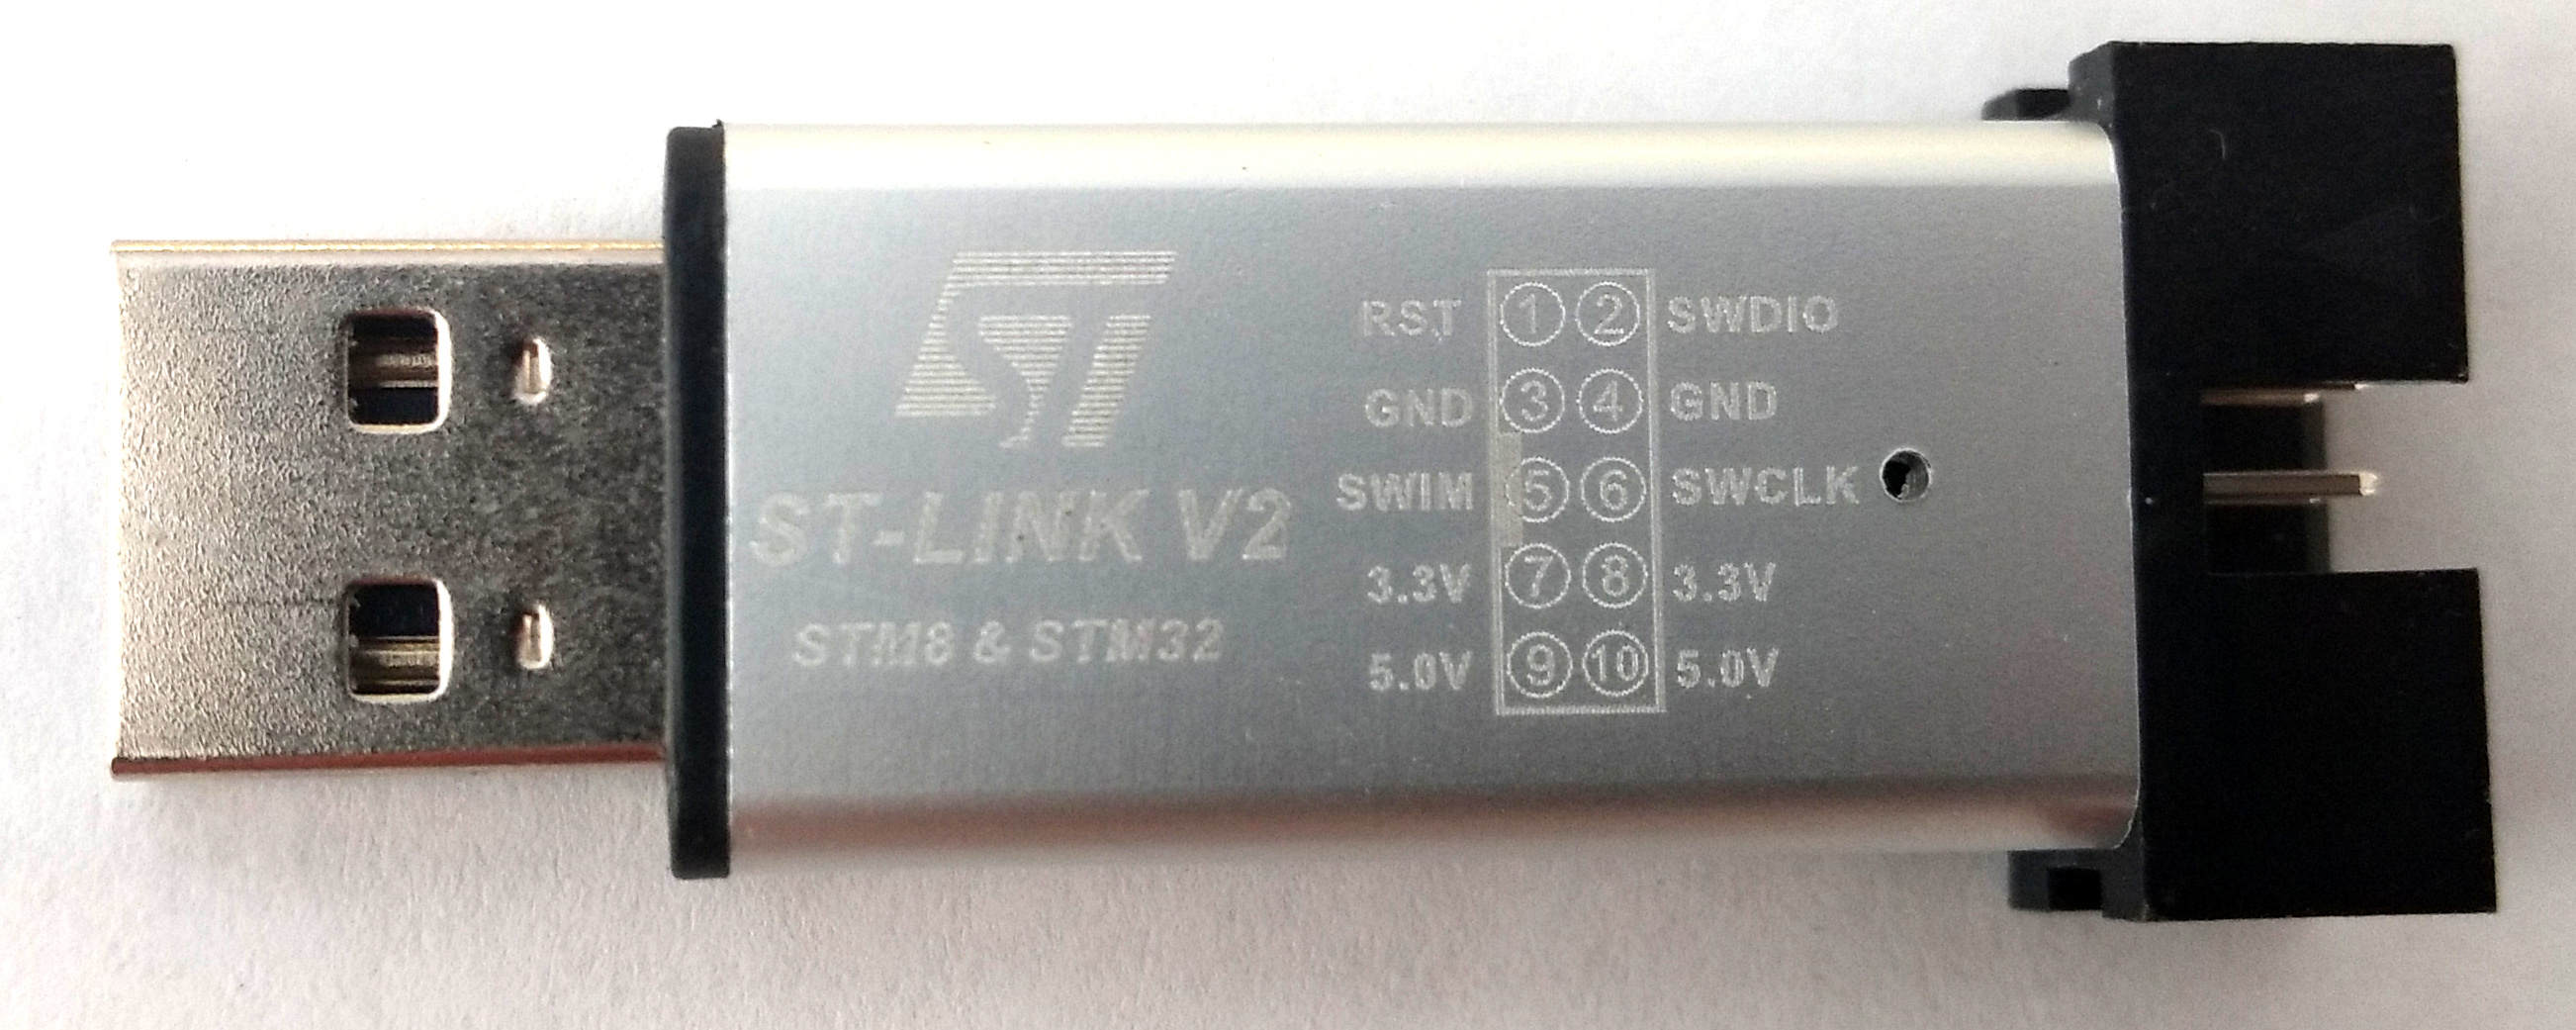
\includegraphics[width=0.7\textwidth]{Figures/st-link-top}}
    \caption{The Chinese ST-Link V2 debug adapter. Note the pinout specification written on the case.}
    \label{fig:stlinktop}
    \end{figure}
    
    \begin{figure}[h!]
    \centering
        \subfloat[Rear view of ST-Link]{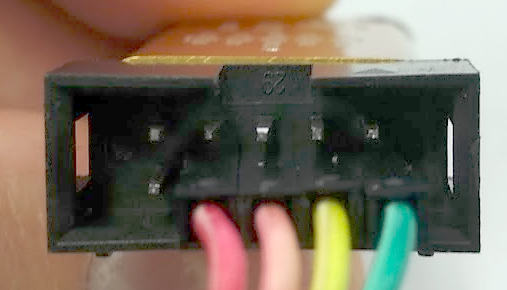
\includegraphics[width=0.4\textwidth]{Figures/stlink_rear}}
        \qquad
        \subfloat[Development board debug header]{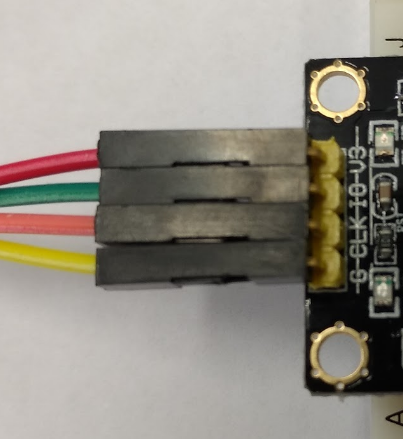
\includegraphics[width=0.4\textwidth]{Figures/stlink_stm32}}
        \caption{Development board debugger connection}
        \label{fig:stm32_debug}
    
    \end{figure}

    \item Connect breadboard GND to one of the STM32 microcontroller's G pins. There are two of these pins, pick whichever is more convenient.
    
    \item Connect a red LED in series with a $330~\Omega$ resistor from pin C13 to GND. Remember that the longer LED pin is the anode (positive) pin and should be facing the GPIO pin.
    
    \item Plug the ST-Link into a free USB port.  
    
\end{enumerate}

\subsection{System Workbench}
\subsubsection{Configuring the Workspace and Importing a Project}

\begin{enumerate}
    \item Download \texttt{STM32Template.zip} from Blackboard.
    
    \item Open System Workbench. If you see a ``Welcome'' screen close it by clicking the X next to the `Welcome' label near the top of the window.
    
    \item System Workbench will prompt you to set a ``workspace'' folder. Choose a folder in your student U:\textbackslash which \textbf{does not contain spaces in the file path}. If the workspace path contains a space character your project will fail to compile.
    
    \begin{figure}[H]
    \centering
    \subfloat[The import type dialog box.]{
        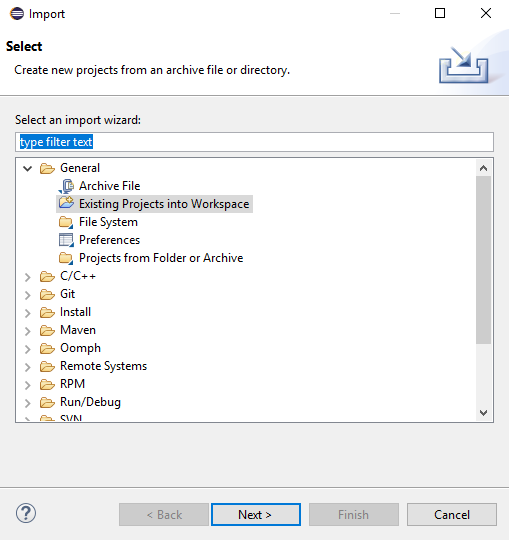
\includegraphics[width=0.48\textwidth]{Figures/importproject}
        \label{fig:importtype}}
    \subfloat[Importing a .zip archive.]{
        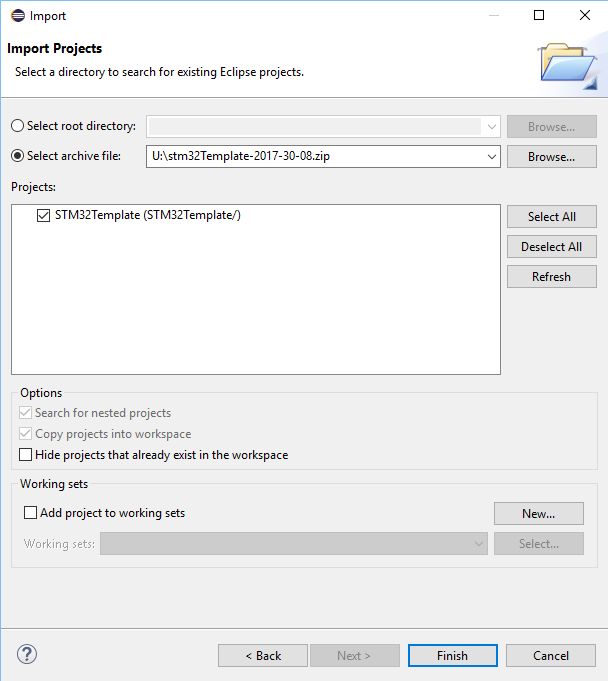
\includegraphics[width=0.48\textwidth]{Figures/importzip}
        \label{fig:importzip}}
    \end{figure}
    
    \item Import the project into the workspace:
    \begin{enumerate}
        \item Click `File \textgreater Import', and select `General \textgreater Existing Projects into Workspace' from the list as shown in Figure \ref{fig:importtype}. Click `Next'.
    
        \item Select the ``Select archive file'' radio button at the top, click `Browse', find \texttt{STM32Template.zip}, and open it. If done correctly you should see something similar to Figure \ref{fig:importzip}.
    
        \item Click `Finish' to close the dialog then ensure that the project exists in the project explorer on the left side of the screen.
    \end{enumerate}
    
    \item Compile the project by typing \texttt{CTRL+B} or clicking through the `Project \textgreater Build All' menu. If this fails do it again 2-3 times or until it finishes without error.
\end{enumerate}

\pagebreak

\subsubsection{Configuring the debug environment}

\begin{enumerate}
    \item Right click on the project name and select ``Debug As \textgreater Debug Configurations...'', as shown in Figure \ref{fig:debugicon}.
    
    \begin{figure}[H]
    \makebox[\textwidth][c]{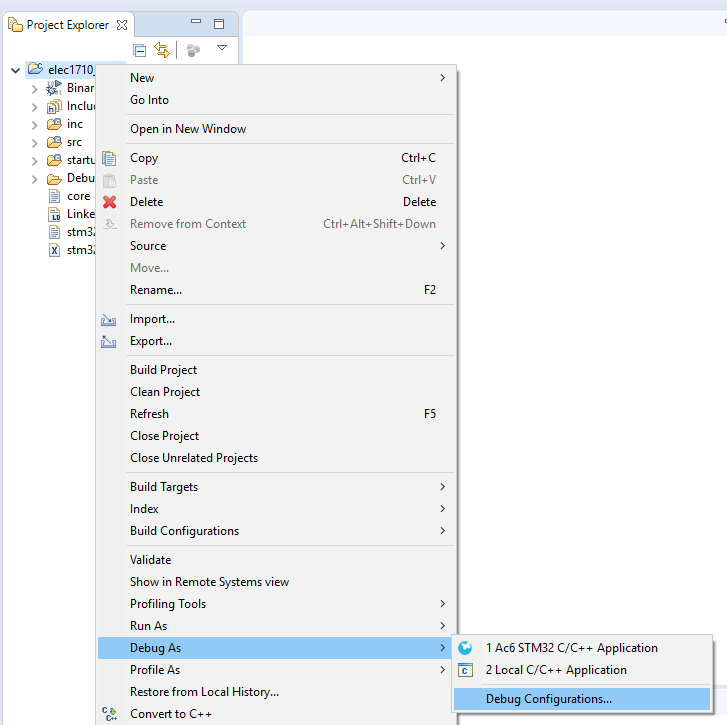
\includegraphics[width=0.65\textwidth]{Figures/opendebugconf}}
    \caption{Opening the debug configuration.}
    \label{fig:debugicon}
    \end{figure}

    \item Highlight `Ac6 STM32 Debugging' and click the `New launch configuration' button (highlighted in Figure \ref{fig:debugconfig}).

    \begin{figure}[H]
    \makebox[\textwidth][c]{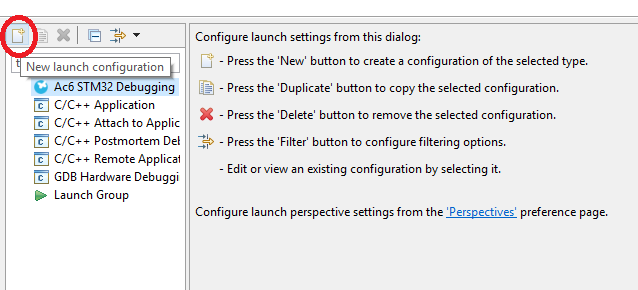
\includegraphics[width=0.65\textwidth]{Figures/ide_debug2}}
    \caption{Creating a new Ac6 STM32 debug configuration.}
    \label{fig:debugconfig}
    \end{figure}


    \item Select the new configuration and navigate to the `main' tab as shown in Figure \ref{fig:debug_noelf}.
    
    If the box under C/C++ Application is empty,  as it is in Figure \ref{fig:debug_noelf}, select 'search project' and choose the binary as shown in  Figure\ref{fig:elf_selection}. After selecting ok the .elf file should now be shown as it is in Figure\ref{fig:elf_filled_in}.
    
    If the \texttt{.elf} file does not appear when clicking `Search Project...' then the project did not compile correctly. Press \texttt{ctrl+b} again or, as a last resort, select the menu item `Project - clean' from the top menus then attempt a build 2 or 3 more times. 
   
    \begin{figure}[H]
    \makebox[\textwidth][c]{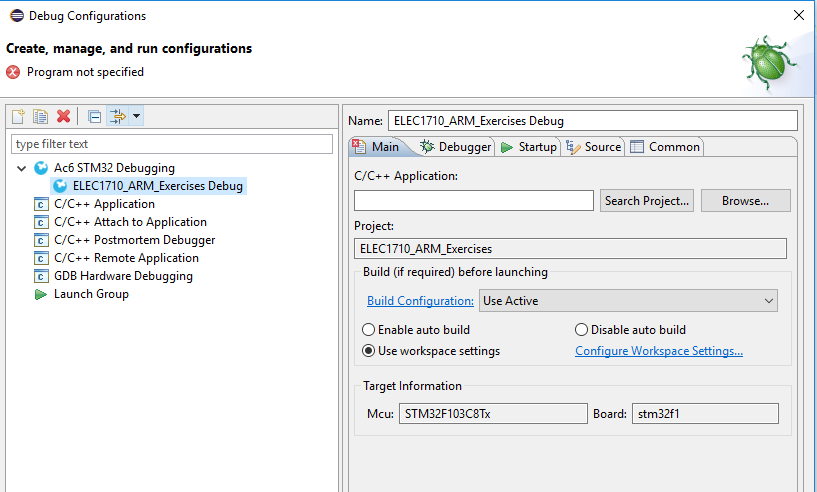
\includegraphics[width=0.7\textwidth]{Figures/debug_noelf}}
    \caption{The debug configuration window.}
    \label{fig:debug_noelf}
    \end{figure}

   \begin{figure}[H]
    \makebox[\textwidth][c]{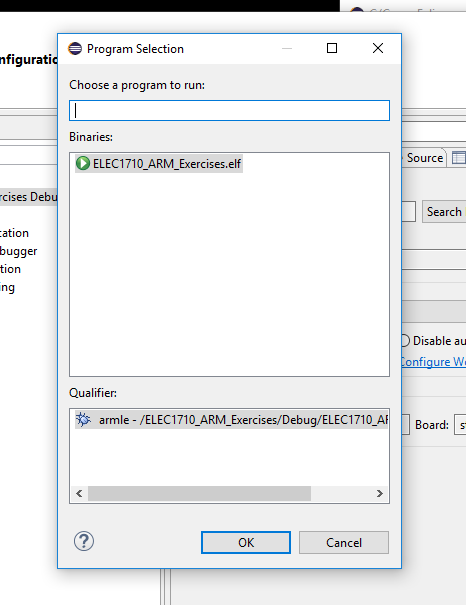
\includegraphics[width=0.7\textwidth]{Figures/elf_selection}}
    \caption{Manually finding the \texttt{.elf} binary file.}
    \label{fig:elf_selection}
    \end{figure}

   \begin{figure}[H]
    \makebox[\textwidth][c]{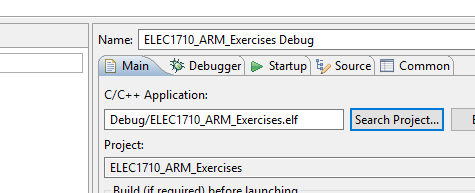
\includegraphics[width=0.7\textwidth]{Figures/elf_filled_in}}
    \caption{A correctly configured `Main' tab.}
    \label{fig:elf_filled_in}
    \end{figure}


    \item Navigate to the `Debugger' tab. Click the ``Show generator options'' button and select ``Software system reset'' from the ``Reset Mode'' drop down menu, as shown in Figure \ref{fig:openocdconfig}).
   
    \begin{figure}[H]
    \makebox[\textwidth][c]{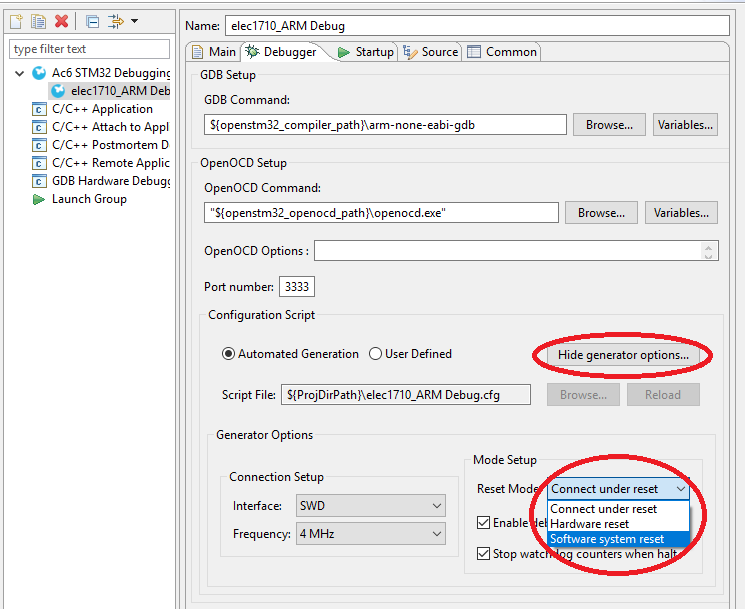
\includegraphics[width=0.7\textwidth]{Figures/debugconf}}
    \caption{Configuring OpenOCD for the ST-Link debugger.}
    \label{fig:openocdconfig}
    \end{figure}

    \item Ensure the ST-Link is plugged into the PC USB port.  Click the `Debug' button (bottom right), this will recompile the project then load the resulting binary onto the STM32 dev board and bring up a dialog box asking if you want to swap to the debug `perspective'. Click yes. You can swap between the debug and C/C++ perspectives by clicking the appropriate icons in the top right of the System Workbench window (ask a demonstrator to help locate them, they are small and subtle).


\end{enumerate}

\pagebreak

\subsubsection{Debugging Code on the STM32}

\begin{enumerate}
    \item Execute the `blinky' code using the debugger functions shown in the video (from 7 mins 10 sec). \textbf{NB:} Pressing the red square will terminate the exection, requiring a debugging session restart. Use the yellow vertical bar `Pause' button to stop execution temporarily.
    
    \begin{itemize}
        \item Use single instruction step mode
        \item Use (\texttt{CTRL+r}) to run to a given line
        \item Use breakpoints (\texttt{CTRL+SHIFT+b}) to stop the execution at a given line
        \item Observe variables and registers in the upper right hand window
        \item Manually modify register and peripheral contents
    \end{itemize}
    
    \item With the code running observe the LED on pin C13 flash
    
    \item \textbf{Task:} Modify the assembly code to blink the LED soldered to the STM32 development board. It is connected to pin B12 (GPIOB, pin 12). See Appendix~\ref{modified}
    \begin{itemize}
        \item \texttt{GPIOB\_ODR} is at address \texttt{0x40010C0C}, add a \texttt{.equ} assembly directive to define this value. Using a \texttt{.equ} increased readability as the text \texttt{GPIOB\_ODR} is used instead of a seemingly cryptic hexadecimal constant.
        \item B12 is set to logic 1 with the constant \texttt{0x00001000}. Modify the appropriate \texttt{ldr} instruction to reflect this. \textbf{NB:} Pins are numbrered starting at zero.
        
        \item The LED is wired in an active low configuration. Setting B12 to a logic 0 turns the LED on.
    \end{itemize}
\end{enumerate}

\pagebreak

\section{Appendix}

\subsection{Blinky Source Code}

\begin{lstlisting}[
caption = Blinky code listing
]
    .syntax unified
    .cpu cortex-m3
    .thumb
    .global blink
    // This defines a constant which is the STM32F103's address for the
    // port C output data register
    .equ	GPIOC_ODR,	0x4001100C
// NB: This function assumes that GPIOC was pre-configured as an output
blink:
	ldr r0, =0x00002000 // The "2" puts a 1 in bit 13, for output pin PC13
	ldr r1, =0x00000000 // A source of zero to turn off PC13
	ldr r2, =GPIOC_ODR  // Load r2 with the address of GPIOC_ODR

	str r0, [r2] 	// Store the contents of r0 into the memory address
			// in r2. This turns on PC13, turning OFF the LED.

	ldr r3, =0x00080000 	// This function counts down from this bit number
delay1:
	sub r3, r3, #1   	// Subtract 1 from r3 and store result back in r3
	cmp r3, #0	// Compare r3 to zero. Sets status flags
	it gt		// IT (if-then) block.
	bgt delay1	// If the comparison result was "greater-than"

	str r1, [r2]	// Store the contents of r1 into the memory address
			// in r2. This turns off all of PORTC turning ON the LED.

	ldr r3, =0x00080000 	// This function counts down from this bit number
delay2:
	sub r3, r3, #1	// Subtract 1 from r3 and store result back in r3
	cmp r3, #0	// Compare r3 to zero. This sets status flags
	it gt		// IT (if-then) block.
	bgt delay2	// If the comparison result was "greater-than"

	b blink		// Branch back to "blink" label
\end{lstlisting}

\newpage

\subsection{Modified Blinky Source Code} \label{modified}

\begin{lstlisting}[
caption = Blinky code listing
]
    .syntax unified
    .cpu cortex-m3
    .thumb
    .global blink
    // This defines a constant which is the STM32F103's address for the
    // port B output data register
   .equ	GPIOB_ODR,  	0x40010C0C

// NB: This function assumes that GPIOC was pre-configured as an output
blink:
          ldr r0, =0x00001000 // The "1" puts a 1 in bit 12, for output pin 12
	ldr r1, =0x00000000 // A source of zero to turn on pin 12
	ldr r2, =GPIOB_ODR  // Load r2 with the address of GPIOB_ODR

	str r0, [r2] 	// Store the contents of r0 into the memory address
			// in r2. This turns on PC12, turning OFF the LED.

	ldr r3, =0x00080000 	// This function counts down from this bit number
delay1:
	sub r3, r3, #1   	// Subtract 1 from r3 and store result back in r3
	cmp r3, #0	// Compare r3 to zero. Sets status flags
	it gt		// IT (if-then) block.
	bgt delay1	// If the comparison result was "greater-than"

	str r1, [r2]	// Store the contents of r1 into the memory address
			// in r2. This turns off all of PORTB turning ON the LED.

	ldr r3, =0x00080000 	// This function counts down from this bit number
delay2:
	sub r3, r3, #1	// Subtract 1 from r3 and store result back in r3
	cmp r3, #0	// Compare r3 to zero. This sets status flags
	it gt		// IT (if-then) block.
	bgt delay2	// If the comparison result was "greater-than"

	b blink		// Branch back to "blink" label
\end{lstlisting}


\pagebreak

\subsection{GPIO Memory Addresses}

In order to calculate the memory addresses of the STM32's GPIO ports several resources need to be consulted. Each GPIO port is configured by multiple registers, each with a unique memory address. However, since each GPIO port (A through to E) has the same set of registers they are not all listed individually. Instead the \textit{base address} of each GPIO port is published in the datasheet and the \textit{offset} of each register from this base address is published in the reference manual.

The base address of \texttt{GPIOC} is shown in Figure \ref{fig:gpioaddr} to be \texttt{0x4001 1000} (likewise \texttt{GPIOB}'s is \texttt{0x4001 0C00}. Figure \ref{fig:gpioodr} then shows that the output data register (\texttt{GPIOx\_ODR}) is found at an offset of \texttt{0x0C} from this base address. So \texttt{GPIOB}'s output data register is at \texttt{0x4001 0C00 $+$ 0x0C $=$ 0x4001 0C0C} and likewise \texttt{GPIOC}'s output data register is at \texttt{0x4001 100C}.



\begin{figure}[H]
\makebox[\textwidth][c]{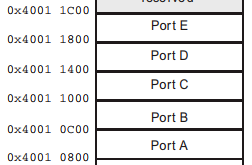
\includegraphics[width=0.4\textwidth]{Figures/stm32_gpio_memory}}
\caption{The GPIO memory base addresses are found in the \textit{memory map}. Extracted from Figure 11 of the STM32F103x8 datasheet.}
\label{fig:gpioaddr}
\end{figure}

\begin{figure}[H]
\makebox[\textwidth][c]{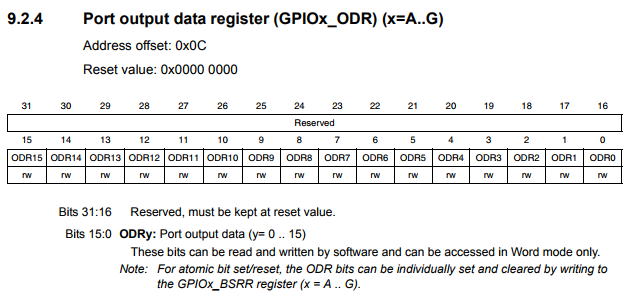
\includegraphics[width=1\textwidth]{Figures/gpio_odr}}
\caption{The \textit{output data register} (\texttt{GPIOx\_ODR}) is listed as having an \textit{offset} of \texttt{0x0C}. Extracted from the reference manual (RM0008).}
\label{fig:gpioodr}
\end{figure}


\end{document}